\documentclass[13pt]{beamer}

\usepackage{amsmath}
\usepackage{graphicx}
\usepackage[utf8]{inputenc}
\usepackage{multicol}
\usepackage{geometry}
\usepackage{booktabs}
\usepackage{centernot}
\usepackage{pgfpages}
\usepackage{tikz}
\usepackage{listings}
\usepackage{xcolor}
\usepackage{dcolumn}

\lstset{ 
  language=R,
  basicstyle=\ttfamily\small,
  keywordstyle=\color{blue},
  stringstyle=\color{red},
  commentstyle=\color{green},
  morecomment=[l]\#,
  frame=single,
  breaklines=true,
  showstringspaces=false,
  frame=none
}


% Note
% \setbeameroption{show notes on second screen}
% \setbeamercolor{note page}{bg=gray, fg=white}
% \setbeamertemplate{note page}{%
%     % adds in bg color
%         \insertvrule{\paperheight}{note page.bg}%
%         \vskip-\paperheight%
%     % changes font color
%         \usebeamercolor[fg]{note page}%
%     % inserts note
%         \insertnote%
% }

% Theme
\usetheme{AnnArbor}
\usecolortheme{beaver}
\setbeamertemplate{blocks}[default]
\setbeamertemplate{itemize items}[ball]
\setbeamertemplate{frametitle continuation}{}
\setbeamertemplate{bibliography item}{}
\setbeamertemplate{footline}{
  \begin{beamercolorbox}[wd=\paperwidth,ht=2.25ex,dp=1ex]{title in head/foot}
    \usebeamerfont{title in head/foot}
    \hspace{1em} \insertshorttitle \hfill \hspace{-18em} \hfill \insertframenumber /\inserttotalframenumber \hspace*{1em}
  \end{beamercolorbox}
}
\beamertemplatenavigationsymbolsempty
\setbeamertemplate{frametitle continuation}[from second][(Cont.)]

\usepackage[backend=biber, style=apa, citestyle=authoryear]{biblatex}
% \addbibresource{ref.bib}

\title[Data breach and bank loan]{
  Do Banks Price Firms’ Data Breaches?
}

\author{
  Henry He Huang \inst{1} \and
  Chong Wang \inst{2}
}

\institute[shortinst]{
  \inst{1} Yeshiva University \and
  \inst{2} The Hong Kong Polytechnic University
}

% Submission history

\date{\today}

% Section header
% \AtBeginSection[]
% {
%     \begin{frame}
%         \frametitle{Table of Contents}
%         \tableofcontents[currentsection]
%     \end{frame}
% }


\begin{document}

\begin{frame}
  \titlepage
  \begin{tikzpicture}[remember picture,overlay]
    \node[anchor=south east,yshift=10mm,xshift=-5mm] at (current page.south east) {%
      \begin{minipage}{.5\textwidth}
        \raggedleft
        \scriptsize\textit{
          Published on TAR: November 2020
        }
      \end{minipage}
    };
  \end{tikzpicture}
\end{frame}

\section{Introduction}

\begin{frame}
  {The story}
  \begin{center}
    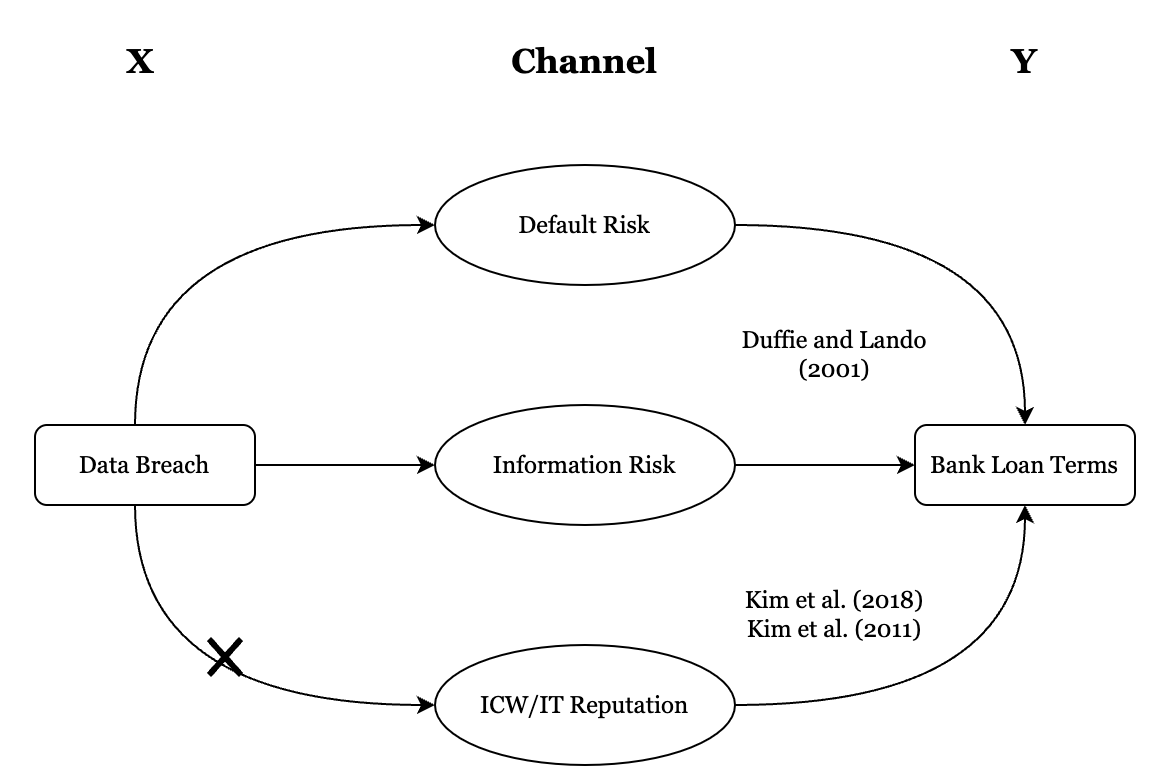
\includegraphics[width=0.8\textwidth]{../figs/hypothesis.png}
  \end{center}
\end{frame}

\section{Replication}

\begin{frame}
  {Sample development}
  \scriptsize
  \begin{table}[ht]
    \centering
    \label{my-label}
    \begin{tabular}{@{}lrr@{}}
      \toprule
      \textbf{Step}                                            & \textbf{Authors'} & \textbf{Mine} \\ \midrule
      \# data breaches from 2005 (2010) to 2014 (2020)         & 551               & 587           \\
      Less:                                                    &                   &               \\
      \quad \# firms with a prior breach event                 & (16)              & (9)           \\
      \quad \# events that are not the most significant        & (70)              & (195)         \\
      \quad \# event firms lacking the data for (PSM)          & (252)             & (155)         \\
      \# event firms after PSM                                 & 213               & 228           \\
      event firms + control firms                              & 426               & 456           \\
      Bank loan observations from 2003 (2008) to 2016 (2022)   & 1,428             & 2165          \\
      Less:                                                    &                   &               \\
      \quad financial services industries                      & (254)             & (166)         \\
      \quad bridge loans and non-fund-based facilities         & (55)              & (NA)          \\
      \quad insufficient to calculate control variables        & (37)              & (26)          \\
      Final sample involving 139 (149) data breach event firms & 1,081             & 1973          \\ \bottomrule
    \end{tabular}
  \end{table}
\end{frame}

\begin{frame}[fragile] % The 'fragile' option is important when using verbatim content like code listings
  \frametitle{Probit Regression}

  \begin{scriptsize}

    \begin{align*}
      \Phi^{-1}(\text{Data Breach Event}_{t}) & =\ \alpha_0 + \alpha_1\text{Firm Size}_{t-1} + \alpha_2\text{Leverage}_{t-1} + \alpha_3\text{ROA}_{t-1} \\
                                              & + \alpha_4\text{Operational Risk}_{t-1} + \alpha_5\text{Tangibility}_{t-1}                              \\
                                              & + \alpha_6\text{Z-score}_{t-1} + \alpha_7\text{MB}_{t-1} + \alpha_8\text{IT Expertise}_{t-1}            \\
                                              & + \alpha_9\text{IT Reputation}_{t-1} + \alpha_{10}\text{Number of Segments}_{t-1}                       \\
                                              & + \alpha_{11}\text{ICW}_{t-1} + \alpha \text{Industry} + \alpha\text{Year} + \varepsilon
    \end{align*}

  \end{scriptsize}

  \rule{\textwidth}{1pt}

  \begin{lstlisting}
  reg_formula <- breach ~ firm_size + leverage + roa + operational_risk + tangibility + z_score + mb + it_expertise + fyear + industry

  ps_model <- glm(reg_formula, data = psm_panel, family = binomial(link = "probit"))
  \end{lstlisting}

\end{frame}


\begin{frame}
  {Probit Regression (Cont.)}
  \scriptsize
  \begin{table}[ht]
    \centering
    \begin{tabular}{@{}lcc@{}}
      \toprule
                                 & Authors'  & Mine     \\
      \midrule
      Firm Size$_{t-1}$          & 0.154***  & 0.182*** \\
      Leverage$_{t-1}$           & -0.016    & 0.199*   \\
      ROA$_{t-1}$                & 0.089***  & -0.164   \\
      Operational Risk$_{t-1}$   & 0.358*    & 0.761    \\
      Tangibility$_{t-1}$        & -0.005    & -0.331*  \\
      Z-score$_{t-1}$            & -0.086    & 0.002    \\
      MB$_{t-1}$                 & -0.000**  & 0.010    \\
      IT Expertise$_{t-1}$       & 0.233***  & -0.024   \\
      IT Reputation$_{t-1}$      & 0.222**   & NA       \\
      Number of Segments$_{t-1}$ & -0.009    & NA       \\
      ICW$_{t-1}$                & -0.134    & NA       \\
      Intercept                  & -7.881*** & -11.895  \\
      \midrule
      Industry/Year              & Included  & Included \\
      Number of Observations     & 57,462    & 33,157   \\
      Pseudo R$^2$               & 0.166     & 0.243    \\
      \bottomrule
    \end{tabular}
  \end{table}

\end{frame}


\begin{frame}
  {Difference in Variables for firms Matched by PSM}
  \scriptsize

  \begin{table}[ht]
    \centering
    \begin{tabular}{@{}lcccc@{}}
      \toprule
      Variable           & Treated       & Control       & Diff.           & p             \\
      \midrule
      Firm Size          & 8.308 (8.846) & 8.190 (8.752) & 0.118 (0.094)   & 0.591 (0.545) \\
      Leverage           & 0.459 (0.653) & 0.485 (0.679) & -0.026 (-0.026) & 0.768 (0.397) \\
      ROA                & 0.122 (0.134) & 0.124 (0.130) & -0.002 (0.003)  & 0.859 (0.693) \\
      Operational Risk   & 0.059 (0.039) & 0.077 (0.036) & -0.018 (0.002)  & 0.137 (0.472) \\
      Tangibility        & 0.431 (0.237) & 0.449 (0.241) & -0.018 (-0.003) & 0.643 (0.881) \\
      Z-score            & 3.245 (4.965) & 2.129 (4.770) & 1.116 (0.196)   & 0.408 (0.809) \\
      MB                 & 2.330 (1.619) & 2.455 (1.552) & -0.125 (0.067)  & 0.859 (0.683) \\
      IT Expertise       & 0.364 (0.123) & 0.341 (0.105) & 0.023 (0.018)   & 0.616 (0.567) \\
      IT Reputation      & 0.092         & 0.083         & 0.009           & 0.735         \\
      Number of Segments & 2.055         & 1.853         & 0.203           & 0.252         \\
      ICW                & 0.028         & 0.009         & 0.018           & 0.154         \\
      \bottomrule
    \end{tabular}
  \end{table}
\end{frame}

\begin{frame}
  {Descriptive statistics}
  \scriptsize
  \begin{table}[ht]
    \centering
    \begin{tabular}{@{}lrr@{}}
      Variable                           & \textbf{Authors' Mean} & \textbf{My Mean} \\
      \midrule
      \textit{Bank Loan Characteristics} &                        &                  \\
      \quad Loan Spread                  & 210.500                & 173.673          \\
      \quad Loan Amount                  & 0.954                  & 1.781            \\
      \quad Maturity                     & 55.310                 & 47.196           \\
      \quad Performance Pricing          & 0.423                  & 0.298            \\
      \quad Secured                      & 0.485                  & 0.276            \\
      \quad Total Covenants              & 3.096                  & 5.104            \\

      \textit{Data Breach Variables}     &                        &                  \\
      \quad Breach                       & 0.543                  & 0.568            \\
      \quad Post                         & 0.475                  & 0.375            \\

      \textit{Firm-Level Variables}      &                        &                  \\
      \quad Firm Size                    & 8.779                  & 9.422            \\
      \quad Leverage                     & 0.503                  & 0.650            \\
      \quad          ROA                 & 0.144                  & 0.136            \\
      \quad Operational Risk             & 0.043                  & 0.032            \\
      \quad Tangibility                  & 0.568                  & 0.285            \\
      \quad Z-Score                      & 2.883                  & 3.966            \\
      \quad MB                           & 2.372                  & 1.329            \\
      \quad IT Expertise                 & 0.391                  & 0.114            \\
    \end{tabular}
  \end{table}
\end{frame}

\begin{frame}[fragile]
  {DiD}
  \begin{scriptsize}
    \begin{align*}
      \text{Loan Contract Terms} & = \beta_0 + \beta_1\text{Data Breach} \times \text{Year}_{-1} + \beta_1\text{Data Breach} \times \text{Year}_{0} \\
                                 & + \beta_1\text{Data Breach} \times \text{Year}_{1} + \beta_1\text{Data Breach} \times \text{Year}_{2}            \\
                                 & + \beta \text{Controls} + \varepsilon
    \end{align*}
  \end{scriptsize}

  \rule{\textwidth}{1pt}

  \begin{lstlisting}
  rhs_formula <- ~ breach:year_pre_1 + breach:year_0 + breach:year_post_1 + breach:year_post_2 + log(loan_amount + 1) + log(loan_maturity + 1) + performance_pricing + firm_size + leverage + roa + operational_risk + tangibility + z_score + mb + it_expertise
  
  model_loan_spread <- plm(update.formula(rhs_formula, log(loan_spread) ~ .), data = did_panel, index = c("Ticker", "loan_year"), model = "within", effect = "twoways") \end{lstlisting}
\end{frame}

\begin{frame}
  {Authors' DiD Result}

  \begin{figure}
    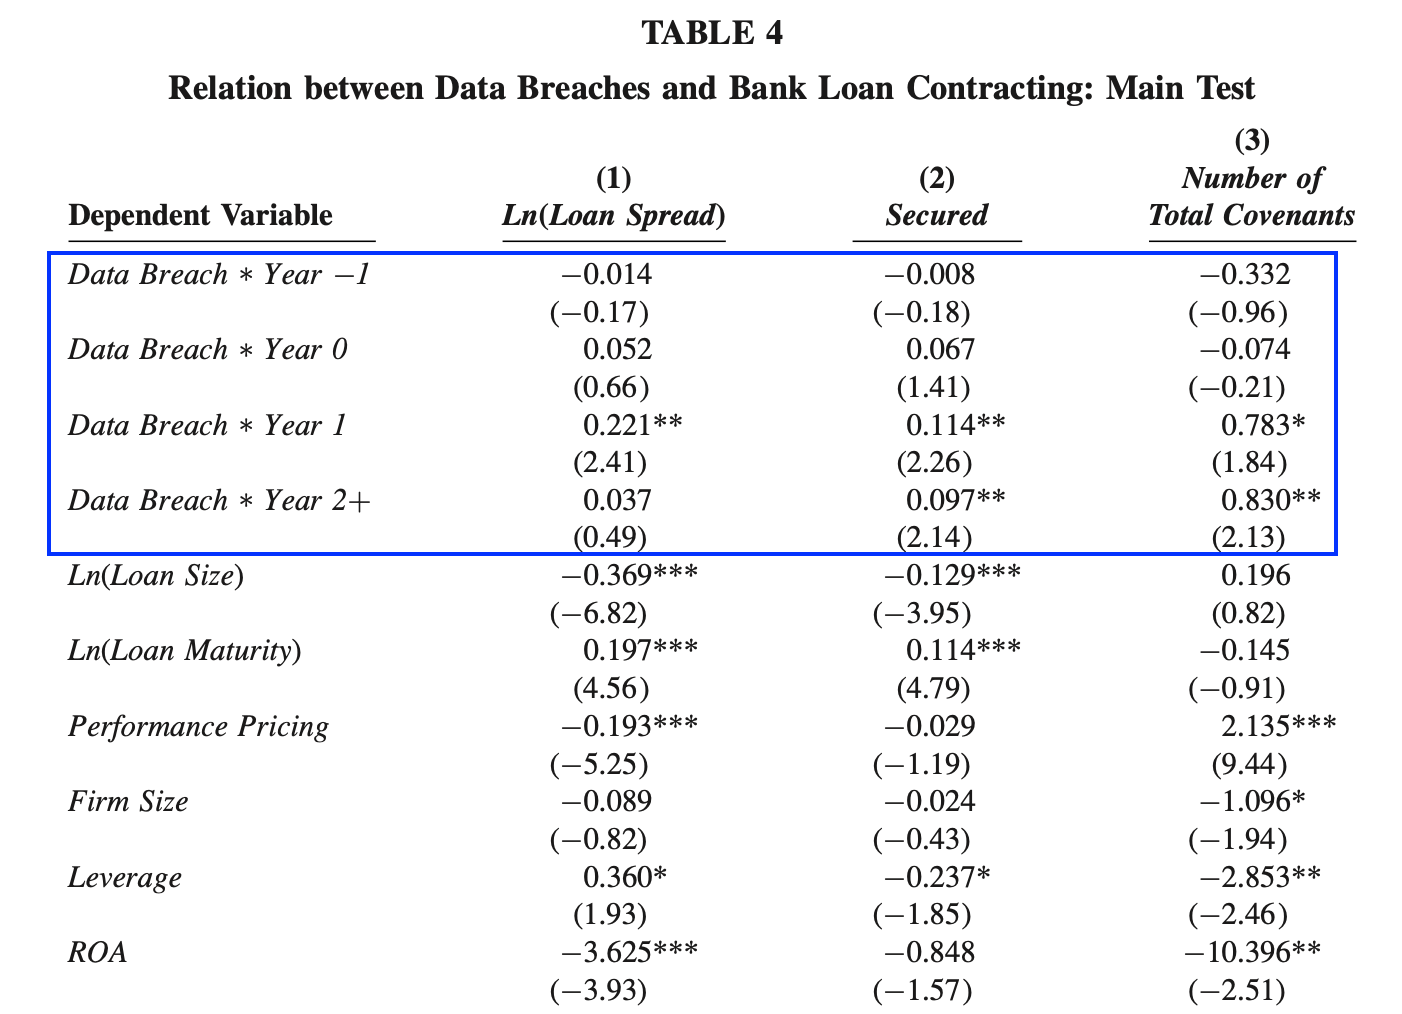
\includegraphics[width=0.8\textwidth]{../tabs/main-result.png}
  \end{figure}
\end{frame}

\begin{frame}{Replication DiD Result}
  \scriptsize
  \begin{table}[!htbp] \centering
    \label{tab:part1}
    \begin{tabular}{@{\extracolsep{5pt}}lD{.}{.}{-3} D{.}{.}{-3} D{.}{.}{-3} }
      \hline
      \hline
                          & \multicolumn{1}{c}{Loan Spread} & \multicolumn{1}{c}{Total Covenants} & \multicolumn{1}{c}{Secured} \\
      \hline
      Breach:Year -1      & 0.009                           & -0.163                              & -0.033                      \\
                          & (0.063)                         & (0.330)                             & (0.041)                     \\
      Breach:Year 0       & -0.010                          & 0.022                               & -0.028                      \\
                          & (0.064)                         & (0.318)                             & (0.041)                     \\
      Breach:Year 1       & -0.031                          & -0.202                              & -0.025                      \\
                          & (0.066)                         & (0.415)                             & (0.045)                     \\
      Breach:Year 2+      & -0.033                          & -0.177                              & 0.008                       \\
                          & (0.045)                         & (0.251)                             & (0.030)                     \\
      Log(Loan Amount)    & -0.018                          & -0.090                              & -0.018^{*}                  \\
                          & (0.016)                         & (0.103)                             & (0.010)                     \\
      Log(Loan Maturity)  & -0.010                          & -0.031                              & 0.066^{***}                 \\
                          & (0.022)                         & (0.124)                             & (0.014)                     \\
      Performance Pricing & 0.082^{***}                     & 0.172                               & 0.043^{**}                  \\
                          & (0.027)                         & (0.136)                             & (0.018)                     \\
      \hline
    \end{tabular}
  \end{table}
\end{frame}

\begin{frame}
  {Replication DiD Result (Cont.)}
  \scriptsize
  \begin{table}[!htbp] \centering
    \label{tab:part2}
    \begin{tabular}{@{\extracolsep{5pt}}lD{.}{.}{-3} D{.}{.}{-3} D{.}{.}{-3} }
      \hline
      \hline
                       & \multicolumn{1}{c}{Loan Spread} & \multicolumn{1}{c}{Total Covenants} & \multicolumn{1}{c}{Secured} \\
      \hline
      Firm Size        & -0.200^{***}                    & -0.365^{*}                          & -0.037                      \\
                       & (0.037)                         & (0.211)                             & (0.024)                     \\
      Leverage         & 0.844^{***}                     & 1.012                               & 0.203^{**}                  \\
                       & (0.128)                         & (0.922)                             & (0.085)                     \\
      ROA              & -1.075^{***}                    & -1.156                              & 0.021                       \\
                       & (0.248)                         & (2.257)                             & (0.168)                     \\
      Operational Risk & 0.309                           & -3.580                              & 0.170                       \\
                       & (0.638)                         & (3.449)                             & (0.418)                     \\
      Tangibility      & 0.309                           & 2.320                               & -0.398^{***}                \\
                       & (0.237)                         & (1.417)                             & (0.154)                     \\
      Z-Score          & 0.029^{*}                       & -0.103                              & -0.012                      \\
                       & (0.016)                         & (0.102)                             & (0.011)                     \\
      MB               & -0.079^{**}                     & 0.094                               & -0.039^{*}                  \\
                       & (0.031)                         & (0.232)                             & (0.021)                     \\
      IT Expertise     & -0.161^{***}                    & 0.120                               & 0.009                       \\
                       & (0.054)                         & (0.288)                             & (0.034)                     \\
      \hline                                                                                                                 \\[-1.8ex]
      Observations     & \multicolumn{1}{c}{1,608}       & \multicolumn{1}{c}{850}             & \multicolumn{1}{c}{1,889}   \\
    \end{tabular}
  \end{table}
\end{frame}
`'
\begin{frame}
  {Conclusion}
  \Large
  Reasons for no results:
  \begin{itemize}
    \item Data breach sample
    \item Control variable
    \item Pattern not generalisable
  \end{itemize}
\end{frame}

\end{document}